\parindent 0 px
\section{\textbf{Analysis}}



\subsection{Statement Of Investigation}
\vspace{15px}
\begin{center}
    \textbf{Can I write a facial recognition algorithm that can be run on video at 15 frames per second?}
\end{center}
\vspace{2px}
\paragraph{I plan to investigate Machine Learning techniques and dynamic programming by developing a facial recognition algorithm in which a program will receive an input of an image and decide whether it is a cat or not.}
\par
\paragraph{To do this I will need to consider what constitutes a successful algorithm, do research into optimisation techniques and understand the mathematics behind the models.}
\par
\paragraph{The program will be tested in the end with a set of test data where I will measure the speed and accuracy of the solution}

\newpage




\subsection{Background}
\par
Machine Learning is a vital part of modern life and more specific object detection and object recognition vastly improve systems in areas such as immigration where facial recognition allows people to be identified autonomously, photography where facial detection can apply effects such as depth of field and filters and in detecting tumours in patients. The applications of this technology will only increase in the future and it may form the basis of the medical screening and security systems so it is important to research new methods and look into optimisation of old ones to future proof our systems. Machine learning works by approximating a classification by adjusting the graph's weights and biases according to how inaccurate the output is. It is important to recognise that the computer doesn't see the face or object but only makes an educated guess on what it is based on the previous examples.
\par

The common methods for facial detection can use the image's texture (the dark and light parts of the object) and structure (the edges on the object) which are identified through matrix operations to form a decision tree or forest that is able to classify the the face. Alternatively, facial detection can be done with neural networks which use a combination of the image's texture and structure of training examples in singular epochs to learn which features make up a face by adjusting the weights and biases of the model in back-propagation.
\par
\text{Examples of }


\subsection{Expert}



\subsection{Interview}

\subsubsection{\textit{Interview Questions}}
\vspace{5px}
\begin{enumerate}
    \item \textbf{Which do you think is more important, the quality of the algorithm or the dataset?}
    \par
    I think with the same dataset different algorithms will learn differently because certain algorithms will tell you how to connect different points together as a mesh and others will do different things so, concerning the end result, an algorithm that is designed specifically for the purpose will run a lot faster and end up only producing what you need which is more memory efficient. More importantly, the dataset you choose will influence what the end result is capable of as, with images that are very blurry, it will be very hard for an algorithm that is trained on 4k images to classify because images in 4k have really well defined edges and they contain lots of information so the dataset is really important for the end result.
    \item \textbf{What approaches are there to facial recognition?}
    \par
    From my experience the main thing is edge detection and edge learning but there are other algorithms out there like eigenfaces or viola-jones.
    \item \textbf{What optimisation techniques have you seen?}
    \par
    You could 1. queue it all up on your own computer or 2. run it on a virtual machine where you can modify the computing power and how much RAM it has to see how fast or slow it is. You should also look into multithreading or code parallelism in the GPU with libraries like OpenCl or Cuda etc...
    \item \textbf{Should I attempt to support multiple bit depths and picture formats?}
    \par
    I dont think so, I think you would make your life a lot harder without really making the end result much better. You would need to have separate algorithms that would be able to digest and support HEIC files for example in the long term so I would stick to files that are very basic. I would stick to files like PNG files because it is very widely used and you would be able to create the algorithm to actually get the file without having to think about the file type very much. If you had the computing power you could to work with raw files but thousands of raw files will take up a huge amount of space and I think it would be a bit over the top.
    \item \textbf{What is the best way of storing and reading from a dataset?}
    \par
    When I was doing my deepfake program I had to match the faces from videos so to store the video I used a folder of a huge amount of images from the video and then ended up having to delete all of the files manually which was quite cumbersome so I would recommend using a folder of temporary files which are files with an expiration of like 1 day for example so then you can automate the process which is a lot easier.
    \item \textbf{What aspects of a program like this do you think make it successful?}
    \par
    If you were google, you would probably produce something that is both accurate and fast but that is obviously very challenging so, in modern industry, I think that consumers want to get the results as fast as possible because we don't have high attention spans like you wouldn't want a super accurate face id that takes 10 minutes to open your phone so I would focus on speed above accuracy where you have acceptable accuracy like at least 90 percent.
    \item \textbf{What should I research before I start programming?}
    \par
    I would suggest looking into google cloud because you can run the programs on their servers which will keep your computer from becoming blocked up and also they have more processing power. My deepfake program was all done on google cloud and it ran surprisingly fast taking like half an hour but it depends because I'd probably just do the small testing data on my own computer.
    \item \textbf{What would you say is the easiest way of tuning my model?}
    \par
    Make sure to output some graphs and graphics of what exactly is happening and what the algorithm is doing to the image so that you can monitor and understand what is going on and change a few things when you see something that is not right because we are by nature graphical learners and outputting numbers to console won't actually mean anything to you.
    \item \textbf{How should I deal with lighting in images where a face in one situation could look completely different in another?}
    \par
    Maybe when you take your input you could mess around with the contrast and try and make it the same as the other images because you how dark it is by looking at the average pixel values. You could also modify your training data so it is composed of a wide range of lighting and quality.
\end{enumerate}

\subsubsection{\textit{Interview Evaluation}}



\newpage

\subsection{Initial Research}

\subsubsection{\textit{Viola Jones Algorithm}}
\text{This approach considers the texture and shading of the object you are trying to identify. It relies on the designer identifying the key features of the object in terms of the areas that are on average darker or lighter than their surroundings in what's called a haar cascade\cite{ViolaJones}. Viola Jones uses } \textbf{AdaBoost} \text{ to generate a forest of stumps that classify the item through each stump’s vote. AdaBoost is a useful algorithm for decision trees as it can turn an array of linear classifications into a non linear form which is useful as data in reality is not always linearly split. For example:}
\par
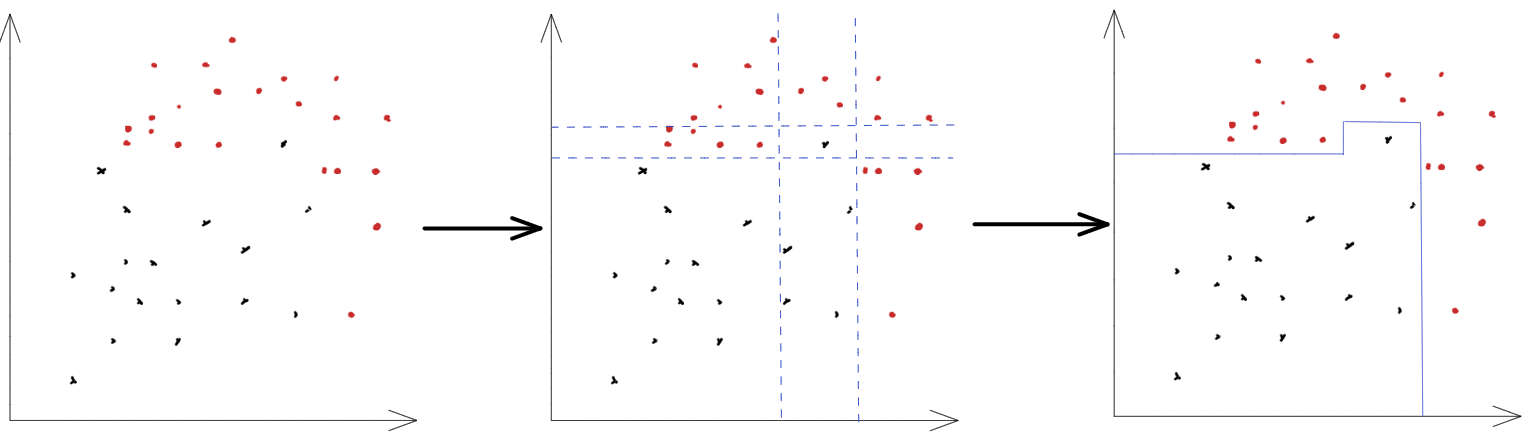
\includegraphics[scale = 0.215]{images/Drawing 2022-05-29 12.03.30.excalidraw.png}

\subsubsection{\textit{AdaBoost}}
\text{AdaBoost is a popular method for training a model based off of decision trees. The steps for AdaBoost are:}
\begin{enumerate}
    \item {Add a new value to each record which is the record’s record weight. This is calculated as $$\frac{1}{Amount \; Of \; Records}$$}
    \item {Generate stumps for each field in the dataset that may or may not be indicative of the correct classification. 'A stump is a tree with just 1 node and 2 leaves'\cite{JoshStarmer}}
    \item Then use the stumps to get the result of each stump’s classification
    \item The stumps will produce a range of values that may or may not be correct for each record. Sum the correct and incorrect classifications for each datapoint in each field and then work out the Gini index which is:
    $$1 - \left[\left(\frac{Amt Identified Correctly}{Total Number Considered}\right)^2 - \left(\frac{Amt Identified Incorrectly}{Total Number Considered}\right)^2\right]$$
    \item The stump with the lowest Gini index is then the most successful stump.
    \item If the stump has a Gini index of 0, that is your correct classifier and the algorithm does not need to run any further. 
    \item Work out the vote for each stump with formula below where the total error is the sum of all of the record weights of the records that the $$Vote = \frac{1}{2} log \left( \frac{1-TotalError}{TotalError} \right)$$\caption{(equation from \cite{JoshStarmer})}
    \item The vote indicates how accurate the stump is where an vote close to 0 says that the field has a 50 percent chance of outputting a correct classification and a positive vote tells us that there is some link between the stump and giving us a correct classification where the larger the number is, the better at classifying the data. A negative vote would therefore indicate that the stump mostly gets it wrong and therefore there may be an inverse relationship between the field and the correct classification.
    \item Then, work out the new record weights of each record. If the record was incorrectly classified by the most successful stump, increase the record weight, if it was correctly classified by the stump, decrease the record weight.
    \begin{itemize}
        \item to increase weight: $$NewWeight = Record Weight \times e^{Vote}$$
        \item to decrease weight: $$New Weight = Record Weight \times e^{-Vote}$$
    \end{itemize}
    \caption{(above equations from \cite{JoshStarmer})}
    \item Then replace the record weights with the new record weights and normalise them by dividing by the sum of all the new record weights. Then start the algorithm from the beginning to get a forest of weak learners that will classify the data.
    \item The forest can be used by running all trees to get those that give a true value as their answer and those that give false, summing the amounts of say of the stumps in each category and choosing the answer that is supported by the largest total vote.
\end{enumerate}

\subsubsection{\textit{Integral Image}}
\text{An integral image is a way of representing an image where each pixel is the sum of all of the pixels before it, this allows us to quickly and efficiently sum all of the values of the pixels in a block and subtract those that came before.}
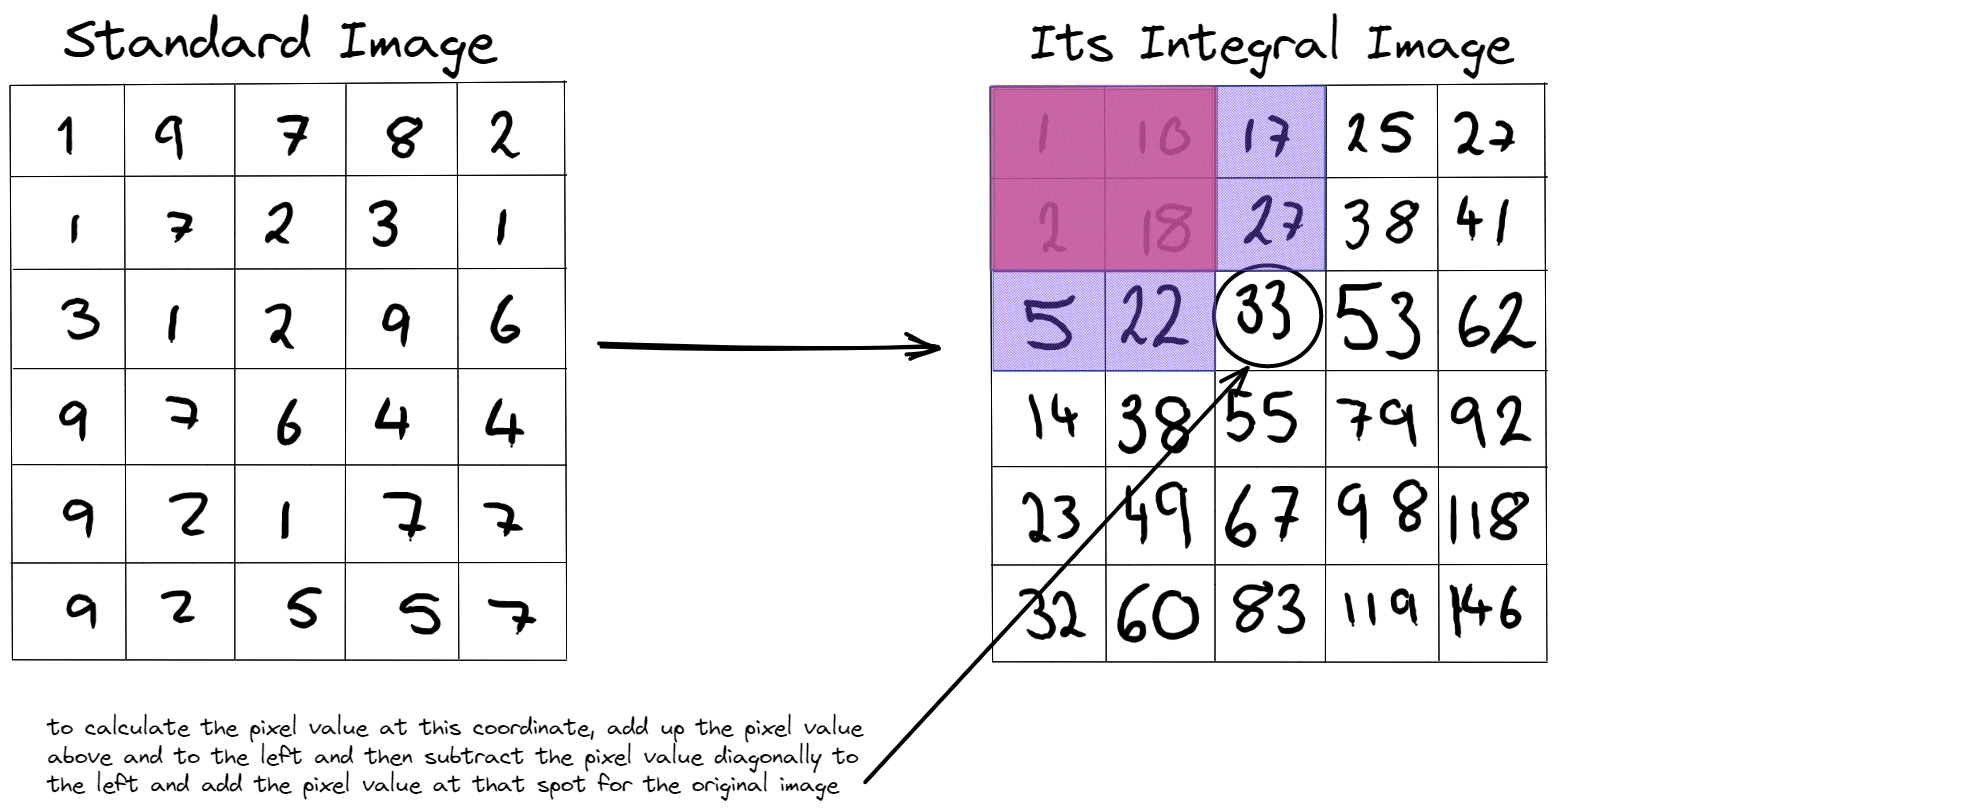
\includegraphics[scale = 0.21]{images/integral image.png}


\subsubsection{\textit{Haar Features}}
\text{Haar features are a substitute to the edge detection kernels and consider the grading of the section compared to another for example a haar kernels could be:}
\begin{center}
    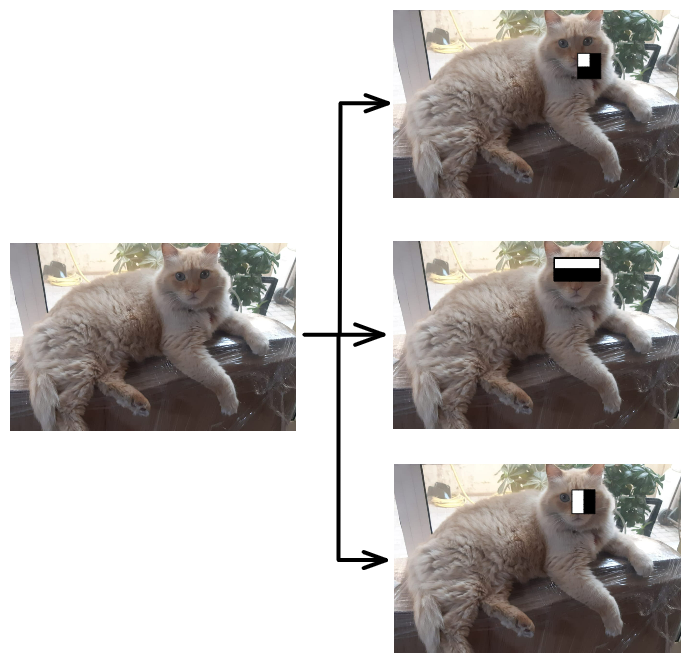
\includegraphics[scale = 0.3]{images/HaarFeatures.png}
\end{center}
\textbf{Computing Haar Feature Extraction:}
\par
\text{we can compute haar features in minimal calculations from an integral image rather than a standard image where you would have to perform many additions and subtractions.}
\hfill
\begin{center}
    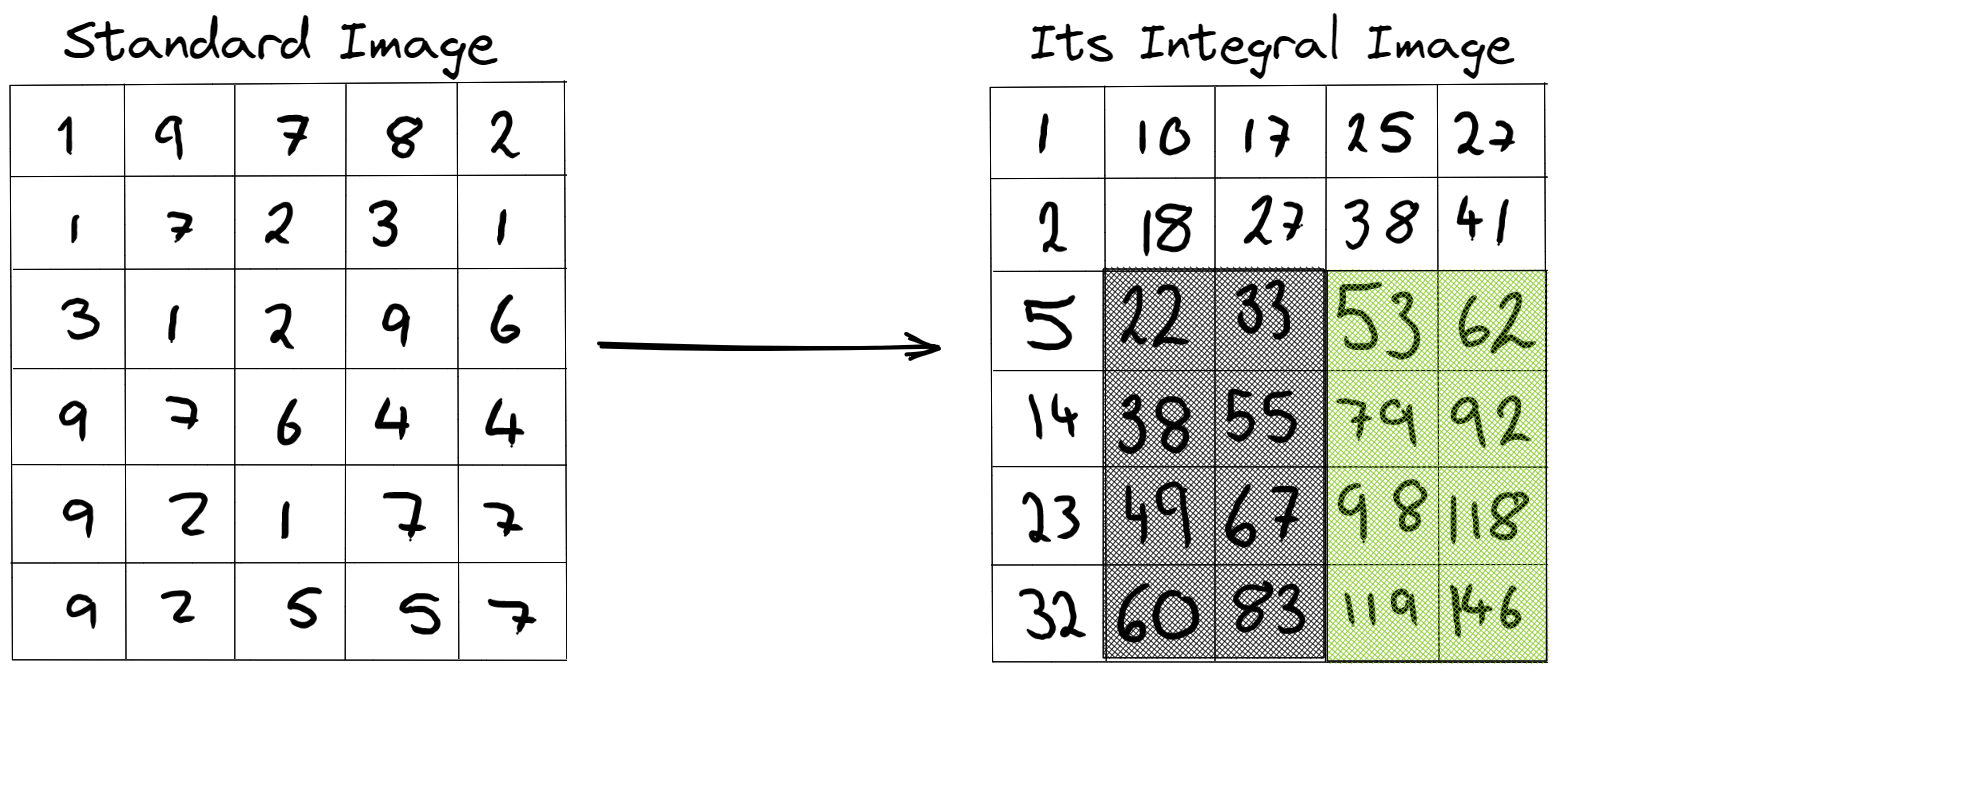
\includegraphics[scale = 0.19]{images/HaarFeatureExtractionV3.png}
\end{center}
\par
\text{to work out the intensity difference of the green section (high intensity section) and the black section (low intensity section) we do:}
\par
\text{$$\left( 83 - 32 - 27 + 2 \right) - \left(146 - 83 - 41 + 27\right) = 23$$}
\par
\text{so the difference between the sections is 23 and therefore this may represent a useful feature. We used 7 operations as opposed to 15 operations in the standard method without an integral image. The amount of operations for a comparison between 2 sections is constant but the amount of comparisons without an integral image scales with the box sizes}

\newpage

\subsubsection{CUDA GPU Programming}
\text{In my project there will be a lot of image processing which means a lot of cycling through pixels or groups of pixels. This means that the time that it takes to run will escalate dramatically and,for example, multiplying kernels on a standard image iteratively has complexity $O\left(n^4\right)$. However, through the use of the Nvidia CUDA libraries, I can exploit GPU parallelism to make these operations run much faster.}
\subsubsection{GPU Architecture}
\text{the modern GPU is split into an array of streaming multiprocessors called a grid. Inside the streaming multiprocessors there are many streaming processors arranged in what is called a block. These streaming processors which we call threads in the programming design have low computational power in comparison to a CPU but there are a lot of them in each block so by splitting our computation into many small operations, we can run these in parallel and get a result much faster. The grids, blocks and threads must be considered while programming in various ways to optimise the program or to produce different results. Connected to the streaming multiprocessors is a section of shared memory called DRAM which is used to store data and in the streaming multiprocessors is a small section of shared memory called the L1 cache. When programming, we must copy the data from host memory on the CPU to device memory on the DRAM and back using the commands, CudaMalloc and CudaMemcpy.}

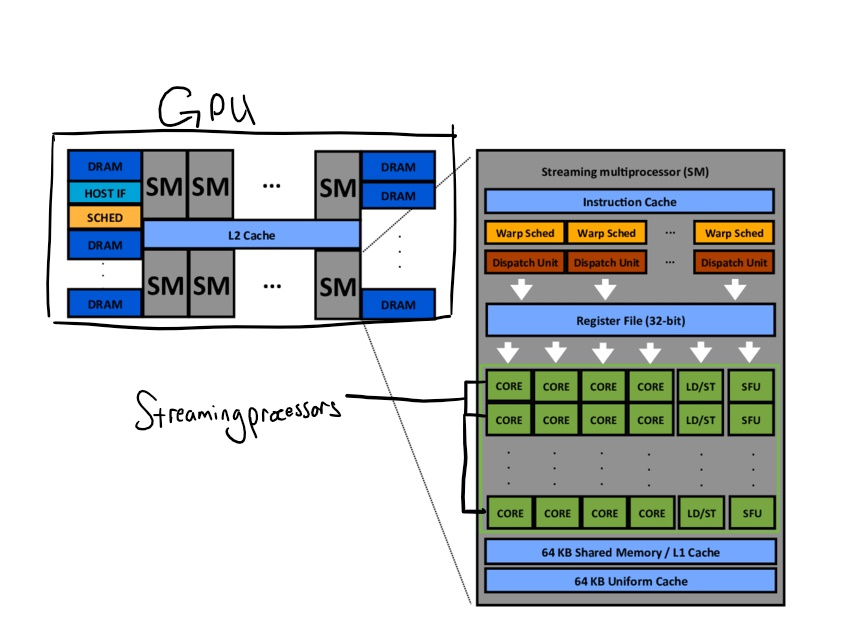
\includegraphics[scale=0.395]{GPUArchV2.jpg}
\cite{GPUArchPhoto}

\subsubsection{CUDA Language and Structure}
\text{First, we start by programming in the host where we initialise all of the variables, set the device, allocate the memory on the GPU copying the data to the registers and set the grid, block and thread sizes. Then we program the kernel which is the code that will be run on all threads. If we are, for example, iterating through pixels in a picture, we assign a thread to each pixel or group of pixels and then locate the thread using the formula: $$index = blockIdx.x \times blockDim.x + threadIdx.x$$ This takes the block index in the x direction and calculates the amount of individual threads by multiplying by the block size in the x direction and then adds on the current thread index in the block. The same formula is used in the y direction switching the 'x's for 'y's so $ blockIdx.x \rightarrow blockIdx.y.$}
\newpage

\subsubsection{EigenFaces}
\begin{itemize}
    \item \textbf{Principal component analysis}:
    \par
    \paragraph{}
\end{itemize}
\subsubsection{FisherFaces}
\begin{itemize}
    \item \textbf{Linear discriminant analysis}:
    \par
    \paragraph{}
\end{itemize}
\subsubsection{\textbf{Potential Data Structures}}
\begin{itemize}
    \item \textbf{graphs}
    \par
    Trees will be important whether I decide to implement a neural network or follow the Viola Jones algorithm. For Viola Jones, I will use decision stumps which are trees composed of a root node connected to 2 nodes where the root node handles the computation and stores the results in the leaf nodes. In the case of a neural network, I will need to build a graph with multiple layers of perceptrons which are nodes that take inputs from many nodes before them to produce an output.
    \item \textbf{square arrays}
    \par
    Square arrays are vital as they allow me to do matrix multiplication efficiently with minimal memory usage as opposed to jagged arrays. They also allow you to copy and pass around data quickly rather than a jagged array which requires more computation copy. In reality, I will probably use a combination of these 2 data structures depending on the use case where, with a jagged array for example, I can quickly extract vectors/single dimensional arrays without need for iteration.
    \item \textbf{structures}
    \par
    I will need to use a structure to preserve the matrix/square array datatype when passing data into my cuda library for matrix multiplication as there are no square arrays in c++. The structure will hold the width of the square array and then hold the data in a 1 dimensional array. I will descend layers in a similar fashion to 2 dimensional arrays but will have to multiply (or divide depending on the situation) the index in the x direction by the layer to access different layers. This is more efficient than using a jagged array as it means I can loop through the array once when resetting it to a square array.
    \item \textbf{queues}
\end{itemize}



\subsection{Prototype}


\subsection{Further Research}


\subsection{Objectives}


\subsection{Modelling Of Problem}

